% !TeX root = 00General.tex
\thispagestyle{standard}
\pagestyle{standard}
\chapter{Ausgangslage}
\label{ausgangs}

Ein Netzwerkmanagement für ein kleines Netzwerk soll eingerichtet werden. Dafür werden die Tools Cacti und Check\_MK verwendet, die auf einer Ubuntu \ac{VM} installiert werden. 
Die Router und Switches sollen mittels \ac{SNMP} überwacht werden. 

Für das Monitoring der Server werden Check\_MK Agents verwendet.


\chapter{Topologie und IP-Adressen}
\label{topo}


Wie in Bild \ref{img:topologie} zu erkennen, wurden für jede Gruppe ein Router mit Switch und den dazugehörigen Servern(\ac{VM}s) in Betrieb genommen.

Unsere Gruppe hatte die Aufgabe den Standort Innsbruck zu betreuen. Dass hei{\ss}t, es wurde das Subnetz mit den \ac{IP} Adressen und dem Gruppenkürzel 5 ausgewählt (z.B. 172.16.5.0/30).


Auf den beiden zur Verfügung gestellten \ac{VM}s, lief jeweils eine Ubuntu 16.04 LTS 64 Bit Version. Für \textbf{Cacti} (siehe Kapitel \ref{cacti}) und \textbf{Check\_MK} (siehe Kapitel \ref{checkmk}) wurden getrennte \ac{VM} verwendet. Näheres dazu in den folgenden Kapiteln.


\begin{figure}[H]
	\centering
	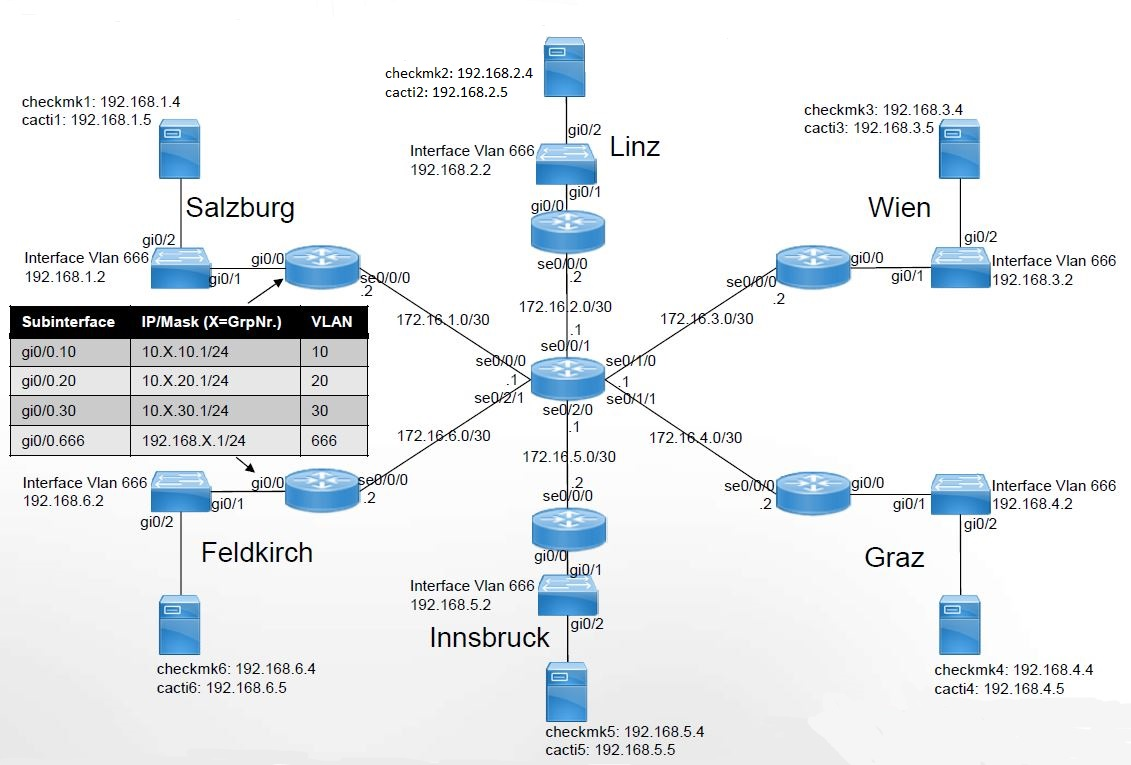
\includegraphics[width=0.9\textwidth]{img/Topologie.JPG}
	\caption{Topologie des Netzwerks (aus Moodle)}
	\label{img:topologie}
\end{figure}

\begin{itemize}
\item IP Adresse: 192.168.5.15 
\item Subnetzmaske: 255.255.255.0
\item Gateway: 192.168.5.1
\item DNS-Server: 193.170.110.64
\item Mit Putty kann per SSH auf den Check\_MK Server (Ubuntu 16.04 LTS 64 Bit) mit der IP 192.168.5.4 zugegriffen werden.
\begin{itemize}
\item Username: nzv
\item Passwort: nzvlab
\end{itemize}
\end{itemize}

\chapter{Switch und Routerkonfiguration}

Auf den Routern und Switches wurde \ac{SNMP} konfiguriert. Der Zugriff sollte auf read-only eingestellt werden. Die Community wurde entsprechend dem zugewiesenen Städtenamen konfiguriert, in diesem Fall "innsbruck".

\section{Switch}

\lstset{escapeinside={\%*}{*)},numbers=left,breaklines}%oder numbers=left
\begin{lstlisting}[caption={SNMP-Config Switch},label={lst:switch},language={}]
snmp-server community innsbruck RO
snmp-server enable traps snmp authentication linkdown 
  linkup coldstart warmstart
snmp-server enable traps transceiver all
snmp-server enable traps call-home message-send-fail 
  server-fail
snmp-server host 192.168.5.4 version 2c innsbruck
\end{lstlisting}

Die Traps werden an den Check\_MK server übertragen.


\section{Router}

Beim Router wurde \ac{SNMP} mitsamt allen Traps aktiviert.

\lstset{escapeinside={\%*}{*)},numbers=left,breaklines}%oder numbers=left
\begin{lstlisting}[caption={SNMP-Config Router},label={lst:router},language={}]
snmp-server community innsbruck RO
snmp-server enable traps snmp authentication linkdown 
  linkup coldstart warmstart
snmp-server enable traps vrrp
snmp-server enable traps transceiver all
...
snmp-server host 192.168.5.4 version 2c innsbruck
\end{lstlisting}

Die Konfiguration ist ähnlich wie schon beim Switch, auch hier werden die Traps an den gleichen Server übertragen.



\chapter{Cacti}
\label{cacti}

Auf dem Ubuntu-Server (IP: 192.168.5.5) wurde Cacti installiert. Die Installation gestaltet sich sehr einfach, da bereits ein Paket vorliegt. 
So genügte \texttt{apt-get install cacti} um Cacti zu installieren.

Im Webinterface wurden anschließend die beiden Netzwerkkomponenten hinzugefügt. Cacti wertet dann die \ac{SNMP}-Werte aus und kann sie grafisch darstellen.

\begin{figure}[H]
	\centering
	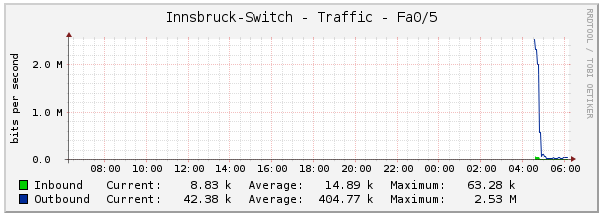
\includegraphics[width=0.9\textwidth]{img/andi_youtube.PNG}
	\caption{Netzwerkauslastung am Switch}
	\label{img:yt}
\end{figure}

In Abbildung \ref{img:yt} sieht man die Auslastung an Port 5 des Switches kurz nachdem ein Video gestreamt wurde. 

\begin{figure}[H]
	\centering
	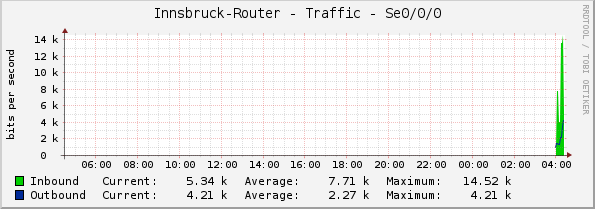
\includegraphics[width=0.9\textwidth]{img/cacti_graph_s00.PNG}
	\caption{Netzwerkauslastung am Router}
	\label{img:uplink}
\end{figure}

Auch der serielle Uplink am Router kann grafisch dargestellt werden, wie in Abbildung \ref{img:uplink} zu sehen ist.

\chapter{Check\_MK}
\label{checkmk}

\section{Switches}

Um nun die EtherChannel Technologie zu realisieren wurden die Ports "FastEthernet 23 und 24" verwendet. Diese werden als sogenannte "Trunk Links" konfiguriert.

\lstset{escapeinside={\%*}{*)},numbers=left,breaklines}%oder numbers=left
\begin{lstlisting}[caption={Setting EtherChannel on a switch},label={lst:etherchannel},language={}]
interface FastEthernet0/24
 switchport trunk allowed vlan 10,20,30
 switchport mode trunk
 channel-protocol lacp
 channel-group 1 mode active
\end{lstlisting}

Des weiteren wurden die verschiedenen \ac{VLAN}s, die auf den jeweiligen Switches hängen, eingestellt.

\lstset{escapeinside={\%*}{*)},numbers=left,breaklines}%oder numbers=left
\begin{lstlisting}[caption={VLAN Konfiguration auf Switch 1},label={lst:vlan},language={}]
interface Vlan10
 ip address 192.168.5.254 255.255.255.0
!
interface Vlan20
 ip address 192.168.15.254 255.255.255.0

\end{lstlisting}

\section{Router}

Als internes Routing Protokoll wurde \ac{OSPF} verwendet. Um \ac{OSPF} richtig zu konfigurieren muss jedem Router eine eindeutige "router-id" zugewiesen werden, sowie alle bekannten Netze in der entsprechenden Area eingetragen werden.

\lstset{escapeinside={\%*}{*)},numbers=left,breaklines}%oder numbers=left
\begin{lstlisting}[caption={OSPF Konfiguration auf Router 1},label={lst:ospf},language={}]
router ospf 10
 router-id 1.1.1.1
 network 10.10.10.0 0.0.0.255 area 0
 network 172.16.5.0 0.0.0.3 area 0
 network 192.168.5.0 0.0.0.255 area 0
 network 192.168.15.0 0.0.0.255 area 0 
\end{lstlisting}

\section{Server}

Nach dem hinzufügen der einzelnen Hardware sowie dem Eintragen der Community Names der anderen Gruppen, konnte eine schöne Übersicht über alle zu überwachenden Geräte angezeigt werden (siehe Bild \ref{img:uebersicht}).

\begin{figure}[H]
	\centering
	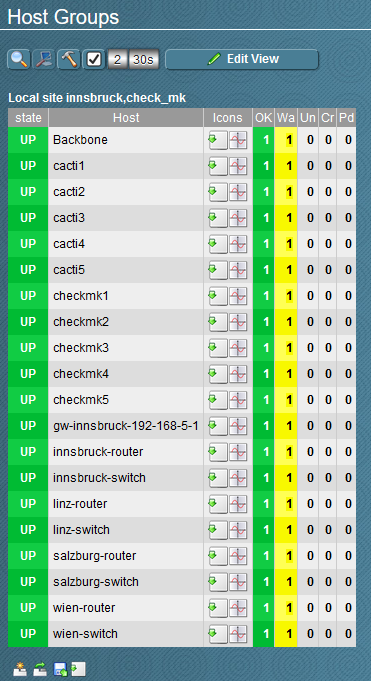
\includegraphics[scale=1]{img/hostgroups.PNG}
	\caption{Übersicht aller gemonitorten Geräte}
	\label{img:uebersicht}
\end{figure}

Zum Anzeigen der vom Router bzw. Switch gesendeten \ac{SNMP}-Traps musste zuvor ein "Ruleset" definiert werden. 
Mit den definierten Rule kann angegeben werden, welche Nachrichten relevant für das Unternehmen/Netzwerk sind und welche Nachrichten ignoriert werden können.


Anschließend können in der Event Console vom Check\_MK Server die \ac{SNMP}-Traps angezeigt werden, wie Bild \ref{img:console} zeigt. Hier zu sehen ist das "down" gehen des FastEthernet Interfaces  05 vom Switch.

\begin{figure}[H]
	\centering
	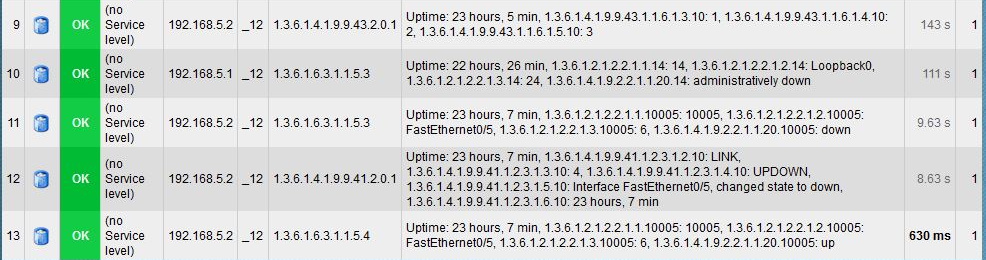
\includegraphics[scale=0.59]{img/EventConsole_cut.PNG}
	\caption{SNMP-Traps vom Router}
	\label{img:console}
\end{figure}

Des weiteren können verschiedene Stati des Routers angezeigt werden (siehe Bild \ref{img:router_monitoring}). Darunter z.B. Temperatur der CPU, den benutzten RAM sowie die angeschlossenen Interfaces.

Diese Traps können wie folgt an den Routern und Switches aktiviert werden:
\begin{lstlisting}[caption={Traps aktivieren},label={lst:traps},language={}]
 snmp-server enable traps
\end{lstlisting}

Die Traps können genau definiert werden, um nur die gewünschten Parameter anzuzeigen. Mit dem oben gelisteten Befehl, werden jedoch alle verfügbaren Parameter übermittelt.

\begin{figure}[H]
	\centering
	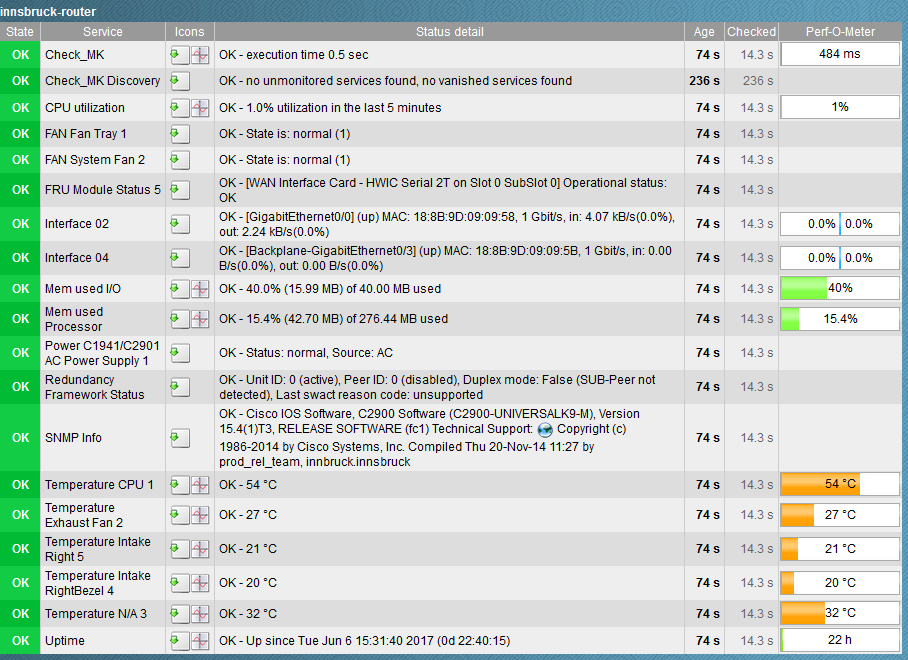
\includegraphics[scale=0.59]{img/checkmk_router.PNG}
	\caption{Stati vom Router}
	\label{img:router_monitoring}
\end{figure}

Ziel war es, alle anderen Gruppengeräte im Netzwerk zu überwachen. Hierfür wurden die \ac{IP} Adressen der anderen Gruppen mit den passenden SNMPv2c Credentials verwendet, um auch diese Parameter abgreifen zu können.


Des weiteren wurde ein Inventory unserer Geräte erstellt, um mittels Check\_MK alle aktiven Interfaces monitoren zu können (siehe Bild \ref{img:inventory_interfaces}).

\begin{figure}[H]
	\centering
	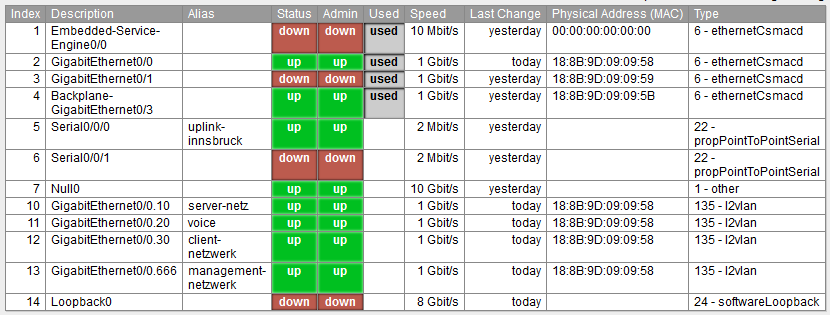
\includegraphics[scale=0.65]{img/inventory_interfaces.PNG}
	\caption{Inventory Interfaces}
	\label{img:inventory_interfaces}
\end{figure}